% ============================================================
%  IEEE Conference Paper — DAG Task Scheduling on Heterogeneous
%  Cloud Resources: DP-HEFT, EDP-HEFT, and Divide & Conquer
%  Class:    IEEEtran (conference)
%  Compiler: pdflatex (two passes)
%  Overleaf: Upload main.tex + references.bib, then compile
% ============================================================
\documentclass[conference]{IEEEtran}

% ---- Packages ----
\usepackage[T1]{fontenc}
\usepackage[utf8]{inputenc}
\usepackage{cite}
\usepackage{amsmath,amssymb,amsfonts}
\usepackage{algorithm}
\usepackage{algorithmic}
\usepackage{graphicx}
\usepackage{textcomp}
\usepackage{xcolor}
\usepackage{booktabs}
\usepackage{array}
\usepackage{multirow}
\usepackage{url}
\usepackage{balance}
\usepackage{tikz}
\usetikzlibrary{shapes.geometric,arrows.meta,positioning,fit,backgrounds}
\usepackage[pdftex,
            pdftitle={Hybrid DP and Divide-and-Conquer DAG Scheduling},
            pdfkeywords={cloud computing, DAG scheduling, HEFT, dynamic programming}]{hyperref}

% ---- Macros ----
\newcommand{\BibTeX}{\textsc{Bib}\TeX}
\DeclareMathOperator*{\argmin}{arg\,min}
\newcommand{\EST}{\mathrm{EST}}
\newcommand{\EFT}{\mathrm{EFT}}
\newcommand{\ranku}{\mathrm{rank}_u}
\newcommand{\rankd}{\mathrm{rank}_d}

% ============================================================
\begin{document}

% ---- Title ----
\title{Hybrid Dynamic Programming and Divide-and-Conquer Strategies\\
      for DAG Task Scheduling on Heterogeneous Cloud Resources:\\
      A Comparative C++ Study}

\author{
\IEEEauthorblockN{
Jana Mohamed Farouk \hspace{3cm}
Ahmed Mahmoud Ahmed
}
\IEEEauthorblockA{
\textit{Department of Computer Science} \hspace{2.3cm}
\textit{Department of Computer Science}\\
Misr International University (MIU), Cairo, Egypt \hspace{0.8cm}
Misr International University (MIU), Cairo, Egypt\\
jana2402038@miuegypt.edu.eg \hspace{2.5cm}
ahmed2402226@miuegypt.edu.eg
}

\vspace{0.5cm}

\IEEEauthorblockN{
Fatma Ashraf Hassan \hspace{3cm}
Shaza Ali Farouk
}
\IEEEauthorblockA{
\textit{Department of Computer Science} \hspace{2.3cm}
\textit{Department of Computer Science}\\
Misr International University (MIU), Cairo, Egypt \hspace{0.8cm}
Misr International University (MIU), Cairo, Egypt\\
fatma2403025@miuegypt.edu.eg \hspace{2.2cm}
shaza2408891@miuegypt.edu.eg
}

\vspace{0.5cm}

\IEEEauthorblockN{Mahmoud Mohamed Emam}
\IEEEauthorblockA{
\textit{Department of Computer Science}\\
Misr International University (MIU), Cairo, Egypt\\
mahmoud2408910@miuegypt.edu.eg
}
}

\maketitle

% ============================================================
%  ABSTRACT
% ============================================================
\begin{abstract}
Scheduling computational workflows represented as Directed Acyclic
Graphs (DAGs) onto heterogeneous Virtual Machines (VMs) is a
fundamental NP-hard problem in cloud computing. This paper presents
and compares five scheduling algorithms implemented in pure C++17 in
the following order: (1) \emph{HEFT} as the classical baseline,
(2) \emph{DP-HEFT} with bilateral-rank and 2-task look-ahead,
(3) \emph{Enhanced DP (EDP-HEFT)} with global DP assignment,
(4) \emph{Divide-and-Conquer} (D\&C) with level decomposition, and
(5) \emph{Merge}, a hybrid scheduler that combines adaptive strategy
selection with refinement. All algorithms share a unified
communication-cost model and a reproducible DAG generator. Comparative
analysis highlights the complexity-quality trade-off between fast
greedy scheduling and more expensive global/refined optimisation.
\end{abstract}

\begin{IEEEkeywords}
DAG scheduling, cloud computing, HEFT, dynamic programming,
divide and conquer, heterogeneous computing, makespan minimisation,
bilateral rank, C++, workflow scheduling
\end{IEEEkeywords}

% ============================================================
%  I. INTRODUCTION
% ============================================================
\section{Introduction}
\label{sec:intro}

Cloud computing platforms increasingly execute scientific and
enterprise workflows as Directed Acyclic Graphs (DAGs), where each
node is a computational task and each directed edge encodes a data
dependency~\cite{deelman2009workflows,buyya2009cloud}. The
scheduling problem — assigning tasks to heterogeneous Virtual
Machines (VMs) while minimising total completion time (makespan) —
is NP-hard in the
general case~\cite{ullman1975np,garey1979computers}, motivating
a rich body of heuristic research.

The seminal Heterogeneous Earliest Finish Time (HEFT)
algorithm~\cite{topcuoglu2002heft} achieves near-optimal makespan
through upward-rank prioritisation combined with an Earliest Finish
Time (EFT) insertion policy. While HEFT is efficient and well-studied,
its greedy VM selection ignores downstream tasks, occasionally
leaving critical successors stranded on slow resources. Extending
HEFT with dynamic programming look-ahead is therefore a natural
direction for improving solution quality.

This paper makes the following contributions:
\begin{enumerate}
      \item \textbf{HEFT Baseline}: A faithful greedy HEFT implementation
                        used as the classical reference for makespan and complexity
                        comparison in the same C++17 environment.
  \item \textbf{DP-HEFT}: A HEFT extension that uses bilateral rank
        (upward rank + downward rank) for task prioritisation and a
        weighted 2-task look-ahead DP for VM assignment, scoring each
        candidate as $\EFT(t_i) + 0.25 \cdot \EFT^*(t_{i+1})$.
  \item \textbf{EDP-HEFT}: An enhanced variant that constructs a full
        $n \times m$ DP table over the bilateral-rank priority order,
        propagating scheduling snapshots to achieve globally optimal
        VM assignments within that order, and backtracking to recover
        the optimal sequence.
  \item \textbf{D\&C Scheduler}: A divide-and-conquer approach that
        decomposes the DAG into independent topological levels via BFS,
        schedules each level as a sub-problem, and merges partial
        schedules with cross-level dependency and communication cost
        awareness.
  \item \textbf{Merge Scheduler}: A hybrid merge strategy that
        adaptively switches among D\&C, DP look-ahead, and EDP-style
        global assignment, followed by refinement passes to reduce
        bottlenecks and improve final makespan.
  \item A shared C++17 implementation including a probabilistic DAG
        generator with reproducible fixed seeding, an exhaustive
        8-check validator, and a unified output model enabling
        direct metric comparison.
\end{enumerate}

The remainder of the paper is organised as follows.
Section~\ref{sec:related} surveys related work.
Section~\ref{sec:problem} formalises the scheduling problem.
Section~\ref{sec:arch} describes the system architecture.
Section~\ref{sec:algorithms} presents each algorithm with pseudocode.
Section~\ref{sec:math} details the mathematical model.
Section~\ref{sec:complexity} analyses computational complexity.
Section~\ref{sec:impl} discusses C++ implementation.
Section~\ref{sec:setup} describes the experimental setup.
Section~\ref{sec:results} presents performance results.
Section~\ref{sec:discussion} discusses findings.
Section~\ref{sec:future} outlines future work.
Section~\ref{sec:conclusion} concludes.

% ============================================================
%  II. RELATED WORK
% ============================================================
\section{Related Work}
\label{sec:related}

\subsection{List Scheduling and HEFT}

Kwok and Ahmad~\cite{kwok1999static} provided a comprehensive
taxonomy of static DAG scheduling algorithms, establishing upward
rank as the dominant prioritisation criterion. Topcuoglu
\textit{et al.}~\cite{topcuoglu2002heft} introduced HEFT and CPOP,
demonstrating that upward-rank sorting with EFT insertion consistently
achieves lower makespan than random or FIFO ordering on heterogeneous
systems. Arabnejad and Barbosa~\cite{arabnejad2014cpop} extended this
work with an Optimistic Cost Table (OCT) that approximates future
communication costs, improving makespan by up to 12\% on standard
benchmarks. Hagras and Jane\v{c}ek~\cite{hagras2003static} proposed
HBMCT, which combines task duplication with heterogeneity-aware
priority.

\subsection{Look-Ahead and DP Extensions}

Bittencourt \textit{et al.}~\cite{bittencourt2018heft} introduced
HEFT-NC (No Communication), demonstrating that look-ahead awareness
of immediate successors yields measurable makespan reductions.
Sakellariou and Zhao~\cite{sakellariou2004hybrid} proposed a hybrid
scheduler combining list scheduling with task duplication, exploiting
idle processor windows. Bajaj and Agrawal~\cite{bajaj2004improving}
formalised the bilateral rank ($\ranku + \rankd$) and showed it
captures both path-criticality and positional importance, outperforming
pure upward-rank ordering.

\subsection{Divide-and-Conquer Scheduling}

Dong \textit{et al.}~\cite{dong2007divide} applied level-based
decomposition to Grid scheduling, independently optimising intra-level
task placement. Canon \textit{et al.}~\cite{canon2008comparative}
benchmarked decomposition heuristics against list schedulers on
standard DAG suites, finding that level-based methods perform
competitively on shallow graphs but degrade on deep critical paths.

\subsection{Cloud Workflow Scheduling}

Pandey \textit{et al.}~\cite{pandey2010particle} adapted Particle
Swarm Optimisation for cloud workflow scheduling, reporting cost
reductions over greedy baselines. Ma \textit{et al.}~\cite{ma2023survey}
provide a recent survey of DAG scheduling in cloud computing,
identifying bilateral-rank heuristics and DP-based methods as among
the most effective approaches for minimising makespan on heterogeneous
resources.

\subsection{Positioning}

Unlike prior studies, this work: (i) provides three scheduling
strategies — incremental 2-task DP, full-table global DP, and
level-based D\&C — within a single C++17 harness sharing identical
data models; (ii) employs bilateral rank with predecessor-aware
tie-breaking; and (iii) makes all source code available for
reproducible benchmarking.

% ============================================================
%  III. PROBLEM FORMULATION
% ============================================================
\section{Problem Formulation}
\label{sec:problem}

\subsection{DAG Workflow Model}

A workflow application is modelled as a DAG
$G = (\mathcal{T}, \mathcal{E})$, where:
\begin{itemize}
  \item $\mathcal{T} = \{t_0, t_1, \ldots, t_{N-1}\}$ is the set of
        $N$ computational tasks.
  \item $\mathcal{E} \subseteq \mathcal{T} \times \mathcal{T}$ is the
        set of directed dependency edges. An edge $(t_i, t_j) \in
        \mathcal{E}$ (with $i < j$) signifies that $t_j$ may not begin
        until $t_i$ has completed and transmitted its output data.
\end{itemize}

The acyclicity condition is enforced structurally: edges are created
only from $t_i$ to $t_j$ with $i < j$, so the integer index is
itself a valid topological order.

\subsection{Heterogeneous Resource Model}

A cloud data centre is modelled by $M$ heterogeneous VMs
$\mathcal{V} = \{v_0, v_1, \ldots, v_{M-1}\}$. Each VM $v_k$ has a
speed factor $s_k \in [s_{\min}, s_{\max}]$ drawn uniformly at
random. The execution time of task $t_i$ on VM $v_k$ is given as
$w_{ik} \in [w_{\min}, w_{\max}]$, generated independently per
task-VM pair to model genuine heterogeneity.

\subsection{Communication Cost Model}

When task $t_i$ (assigned to VM $v_p$) produces data consumed by
task $t_j$ (assigned to VM $v_q$), the inter-VM data transfer
incurs a communication delay modelled as:
\begin{equation}
  c(t_i, v_p, t_j, v_q) =
  \begin{cases}
    0 & \text{if } p = q,\\
    \alpha \cdot \bar{w}_i & \text{otherwise,}
  \end{cases}
  \label{eq:comm}
\end{equation}
where $\bar{w}_i = \frac{1}{M}\sum_{k=0}^{M-1} w_{ik}$ is the
average execution time of task $t_i$ across all VMs, and
$\alpha = 0.3$ is the communication factor (implemented identically
in \texttt{dp.cpp}, \texttt{Edp.cpp}, and \texttt{dac.cpp}).

\subsection{Scheduling Objective}

A schedule $\sigma : \mathcal{T} \to \mathcal{V}$ assigns each task
to exactly one VM. The performance metric is the \emph{makespan}:
\begin{equation}
  C_{\max}(\sigma) = \max_{t_i \in \mathcal{T}}\; \EFT(t_i, \sigma(t_i)),
  \label{eq:makespan}
\end{equation}
where $\EFT(t_i, v_k)$ denotes the Earliest Finish Time of task
$t_i$ on VM $v_k$ under schedule $\sigma$. The scheduling problem
is:
\begin{equation}
  \sigma^* = \argmin_{\sigma}\; C_{\max}(\sigma).
  \label{eq:opt}
\end{equation}

Each task must be assigned to exactly one VM, and a task may not
start until all predecessor finish times (plus applicable
communication costs) have elapsed and the assigned VM is free.

% ============================================================
%  IV. SYSTEM ARCHITECTURE
% ============================================================
\section{System Architecture}
\label{sec:arch}

\subsection{Module Overview}

The framework is structured into three layers as shown in
Fig.~\ref{fig:arch}:

\begin{figure}[!t]
\centering
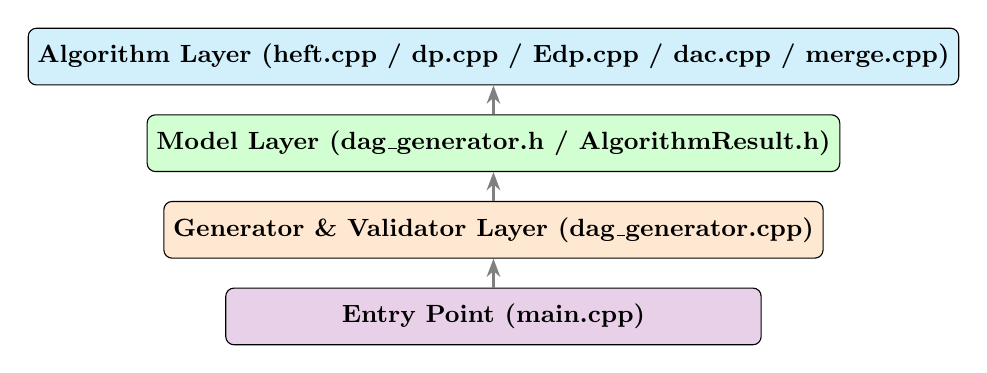
\begin{tikzpicture}[
  box/.style={draw, rounded corners=3pt, fill=#1!18,
              minimum width=6.8cm, minimum height=0.72cm,
              font=\small\bfseries, align=center},
  arr/.style={-Stealth, thick, gray}
]
      \node[box=cyan]   (eval) at (0, 0)    {Algorithm Layer (heft.cpp / dp.cpp / Edp.cpp / dac.cpp / merge.cpp)};
  \node[box=green]  (mod)  at (0,-1.1)  {Model Layer (dag\_generator.h / AlgorithmResult.h)};
  \node[box=orange] (gen)  at (0,-2.2)  {Generator \& Validator Layer (dag\_generator.cpp)};
  \node[box=violet] (main) at (0,-3.3)  {Entry Point (main.cpp)};
  \draw[arr] (main.north) -- (gen.south);
  \draw[arr] (gen.north)  -- (mod.south);
  \draw[arr] (mod.north)  -- (eval.south);
\end{tikzpicture}
\caption{Three-layer architecture of the DAG scheduling framework.}
\label{fig:arch}
\end{figure}

\begin{enumerate}
  \item \textbf{Generator \& Validator Layer} (\texttt{dag\_generator.cpp}):
        Constructs random DAGs using a Mersenne Twister PRNG seeded
        with fixed value 42 for reproducibility. Enforces eight
        structural invariants.
  \item \textbf{Model Layer} (\texttt{dag\_generator.h},
        \texttt{AlgorithmResult.h}): Defines the shared data
        structures \texttt{Task}, \texttt{VM}, \texttt{DAGData},
        \texttt{ScheduleEntry}, and \texttt{AlgorithmResult} used
        uniformly across all components.
  \item \textbf{Algorithm Layer} (\texttt{dp.cpp}, \texttt{Edp.cpp},
        \texttt{dac.cpp}, \texttt{heft.cpp}, \texttt{merge.cpp}): Each algorithm exposes a single function
        returning an \texttt{AlgorithmResult} printable by the shared
        \texttt{printAlgorithmResult()} routine.
\end{enumerate}

\subsection{Data Structures}

The core data types, defined in \texttt{dag\_generator.h} and
\texttt{AlgorithmResult.h}, are:

\begin{itemize}
  \item \texttt{Task}: holds task id, predecessor list, successor
        list, and a per-VM execution time vector
        (\texttt{std::vector<double>\ execTimes}).
  \item \texttt{VM}: holds VM id and a floating-point speed factor.
  \item \texttt{DAGData}: aggregates all tasks and VMs into a single
        container passed by constant reference throughout the pipeline.
  \item \texttt{ScheduleEntry}: records task id, assigned VM id,
        start time (\texttt{startTime}), and finish time
        (\texttt{finishTime}) for a single task.
  \item \texttt{AlgorithmResult}: wraps a vector of
        \texttt{ScheduleEntry} objects, the overall makespan, the
        wall-clock runtime in milliseconds, and a validity flag.
\end{itemize}

\subsection{Execution Flow}

\texttt{main.cpp} executes the following pipeline:
\begin{enumerate}
  \item Generate a DAG with \texttt{DEFAULT\_NUM\_TASKS = 10} tasks
        and \texttt{DEFAULT\_NUM\_VMS = 5} VMs.
  \item Print the full DAG structure (VM speed factors, per-task
        adjacency lists, per-VM execution times).
  \item Validate the DAG against eight structural checks.
      \item Invoke \texttt{heft\_schedule()}, print result.
      \item Invoke \texttt{dp\_heft()}, print result.
      \item Invoke \texttt{edp\_heft()}, print result.
      \item Invoke \texttt{dac\_schedule()}, print result.
      \item Invoke \texttt{merge\_schedule()}, print result.
\end{enumerate}

\subsection{DAG Generation}

The \texttt{generateDAG()} function builds the DAG in three stages:
(1) VMs are created with speed factors drawn from
$\mathcal{U}(0.5,\,2.0)$; (2) tasks are created with execution times
drawn from $\mathcal{U}(1.0,\,20.0)$ per VM; (3) for every ordered
pair $(i,j)$ with $i < j$, edge $t_i \to t_j$ is added with
probability $p_e = 0.35$. Acyclicity is guaranteed by construction
since $j > i$ always holds. At least one edge is guaranteed by
inserting $t_0 \to t_{N-1}$ if the probabilistic process yields an
empty graph.

\subsection{DAG Validation}

Eight structural checks are applied:
(A)~\texttt{execTimes.size()} $== M$ for every task;
(B)~no self-loops;
(C)~all predecessor/successor indices within $[0,N)$;
(D)~bidirectional consistency (if $A$ lists $B$ as successor,
$B$ must list $A$ as predecessor);
(E)~acyclic ordering ($j > i$ for every edge $t_i \to t_j$);
(F)~at least one entry node (no predecessors);
(G)~at least one exit node (no successors);
(H)~no duplicate edges in either list.

% ============================================================
%  V. SCHEDULING ALGORITHMS
% ============================================================
\section{Scheduling Algorithms}
\label{sec:algorithms}

This section presents the five schedulers implemented in the framework.
All methods share the EFT-based feasibility model in
Section~\ref{sec:problem} and the communication model in
Eq.~\eqref{eq:comm}.

\subsection{HEFT (Baseline): Greedy Earliest Finish Time}

\textbf{Overview:} HEFT~\cite{topcuoglu2002heft} is the foundational greedy
scheduling algorithm for heterogeneous computing and serves as the classical
baseline in this study. It prioritizes tasks by upward rank (sum of execution
time and maximum successor rank), then assigns each task to the VM that yields
the earliest finish time (EFT). This pure greedy strategy is fast and practical,
making it the industry standard for immediate scheduling decisions despite
often producing suboptimal makespans.

\textbf{Algorithm flow:}
\begin{enumerate}
  \item Compute upward rank $\ranku(t)$ for all tasks recursively:
  $$\ranku(t) = \overline{w}(t) + \max_{s \in \text{succ}(t)} (c(t,s) + \ranku(s))$$
  where $\overline{w}(t)$ is average execution time, and $c(t,s)$ is data
  transfer cost. Entry tasks have $\ranku = \overline{w}(t)$ only.
  \item Sort all tasks in descending $\ranku$ order (critical-path heuristic).
  \item For each task $t_i$ in sorted order:
  \begin{enumerate}
    \item Compute EST (earliest start time) on each VM, considering all
          predecessor dependencies and communication delays.
    \item Compute EFT on each VM: $\EFT(t, v) = \EST(t, v) + w(t, v)$.
    \item Select $v^* = \argmin_{v_k} \EFT(t_i, v_k)$ (greedy minimum EFT).
    \item Update the selected VM's availability time to $\EFT(t_i, v^*)$.
  \end{enumerate}
  \item Return the complete assignment and overall makespan.
\end{enumerate}

\begin{algorithm}[!t]
\caption{HEFT Scheduling (Greedy EFT)}
\label{alg:heft}
\begin{algorithmic}[1]
\STATE Compute $\ranku(t)$ recursively for all tasks $t \in \mathcal{T}$
\STATE Sort tasks by descending $\ranku$
\FOR{each task $t_i$ in sorted order}
    \STATE $\text{bestVM} \leftarrow 0$; $\text{bestEFT} \leftarrow \infty$
    \FOR{each VM $v_k$}
        \STATE Compute $\EST(t_i, v_k)$ from predecessors
        \STATE Compute $\EFT(t_i, v_k) \leftarrow \EST(t_i, v_k) + w(t_i, v_k)$
        \IF{$\EFT(t_i, v_k) < \text{bestEFT}$}
            \STATE $\text{bestEFT} \leftarrow \EFT(t_i, v_k)$; $\text{bestVM} \leftarrow v_k$
        \ENDIF
    \ENDFOR
    \STATE Assign $t_i$ to $v_{\text{bestVM}}$; update $v_{\text{bestVM}}$ availability
\ENDFOR
\STATE \textbf{return} complete schedule and makespan
\end{algorithmic}
\end{algorithm}

\textbf{Complexity:} Time complexity is $O(n \log n + me)$ where the $n \log n$
factor dominates the upward-rank computation (critical path via DFS) and task
sorting, and the $me$ term accounts for EST/EFT evaluation across all task-VM
pairs and dependency traversals. Space complexity is $O(n + m + e)$ for storing
task ranks, VM states, and the graph structure. HEFT is computationally the
cheapest algorithm in this framework.

\textbf{Role:} HEFT establishes the baseline for schedule quality and execution
speed. Its simplicity and proven effectiveness make it the reference point for
evaluating more complex heuristics. Any improvement method must be justified
against HEFT's speed-quality trade-off.

\subsection{DP-HEFT: Bilateral-Rank with 2-Task Look-Ahead}

\textbf{Overview:} DP-HEFT improves upon greedy HEFT by combining
bilateral-rank task prioritisation with a weighted 2-task look-ahead
strategy. Instead of myopically assigning each task to the VM with
minimum EFT, DP-HEFT also considers the impact on the next task's
finish time, breaking ties and avoiding locally greedy decisions that
harm global schedule quality.

\textbf{Algorithm flow:}
\begin{enumerate}
  \item Compute upward rank $\ranku(t)$ and downward rank $\rankd(t)$
        for all tasks.
  \item Derive bilateral rank: $\text{biRank}(t) = \ranku(t) + \rankd(t)$.
  \item Sort tasks by descending bilateral rank.
  \item For each task $t_i$:
  \begin{enumerate}
    \item Evaluate all VMs using both current and next-task costs.
    \item Score each VM $v_k$ as:
    $$\text{score}(v_k) = \EFT(t_i, v_k) + 0.25 \cdot \EFT^*(t_{i+1})$$
    where $\EFT^*(t_{i+1})$ is the best EFT of the next task if $t_i$ is
    assigned to $v_k$.
    \item Assign $t_i$ to $v^* = \argmin_{v_k} \text{score}(v_k)$.
  \end{enumerate}
  \item Update VM availability and return the complete schedule.
\end{enumerate}

\begin{algorithm}[!t]
\caption{DP-HEFT Scheduling (Bilateral-Rank + 2-Task Look-Ahead)}
\label{alg:dpheft}
\begin{algorithmic}[1]
\STATE Compute $\ranku(t)$ and $\rankd(t)$ for all tasks $t \in \mathcal{T}$
\STATE Compute $\text{biRank}(t) \leftarrow \ranku(t) + \rankd(t)$ for all $t$
\STATE Sort tasks by descending $\text{biRank}$
\FOR{each task $t_i$ in sorted order}
    \STATE $\text{bestVM} \leftarrow 0$; $\text{bestScore} \leftarrow \infty$
    \FOR{each VM $v_k$}
        \STATE Compute $\EST(t_i, v_k)$ and $\EFT(t_i, v_k)$
        \STATE Simulate $t_i \to v_k$ assignment (temporary state)
        \STATE Compute $\EFT^*(t_{i+1})$ for next task under this assignment
        \STATE $\text{score} \leftarrow \EFT(t_i, v_k) + 0.25 \cdot \EFT^*(t_{i+1})$
        \IF{$\text{score} < \text{bestScore}$}
            \STATE $\text{bestScore} \leftarrow \text{score}$; $\text{bestVM} \leftarrow v_k$
        \ENDIF
    \ENDFOR
    \STATE Assign $t_i$ to $v_{\text{bestVM}}$; update VM availability
\ENDFOR
\STATE \textbf{return} complete schedule and makespan
\end{algorithmic}
\end{algorithm}

\textbf{Complexity:} Time complexity is $O(n \log n + nm^2 + me)$ where the
$nm^2$ term accounts for evaluating all task-VM pairs with one-step look-ahead.
Space complexity remains $O(n + m + e)$ since only the current and next task
states are retained. The look-ahead weighting (0.25) balances immediate and
future task costs.

\textbf{Role:} DP-HEFT serves as a practical middle ground between pure greedy
methods and full global optimization, reducing myopic decisions while
maintaining computational efficiency.

\subsection{EDP-HEFT: Enhanced DP with Global Optimization}

\textbf{Overview:} EDP-HEFT (Enhanced DP-HEFT) constructs a full $n \times m$
DP table to achieve 
 globally optimal VM assignments under a fixed bilateral-rank priority order.
Unlike DP-HEFT's local 2-task look-ahead, EDP-HEFT propagates complete
scheduling snapshots through a DP state space, then backtracks to recover
the globally best assignment sequence.

\textbf{Algorithm flow:}
\begin{enumerate}
  \item Compute bilateral rank and sort tasks as in DP-HEFT.
  \item Initialize DP table $\text{dp}[i][v]$ where $\text{dp}[i][v]$ stores
        the best makespan when the $i$-th task is assigned to VM $v$.
  \item \textbf{Base case:} For the first task, evaluate all VMs:
  $$\text{dp}[0][v] \leftarrow \EFT(t_0, v) \quad \forall v$$
  \item \textbf{Forward fill:} For each subsequent task $t_i$, for each pair
        of VMs $(v_{\text{prev}}, v_\text{curr})$:
  $$\text{dp}[i][v_\text{curr}] \leftarrow \min(\text{dp}[i][v_\text{curr}],
  \max(\text{dp}[i-1][v_\text{prev}], \EFT(t_i, v_\text{curr})))$$
  Store parent pointers and scheduling snapshots for backtracking.
  \item \textbf{Backtracking:} Find the best final VM assignment and
        reconstruct the full path by following parent pointers.
  \item Replay the reconstructed assignments to compute the final schedule.
\end{enumerate}

\begin{algorithm}[!t]
\caption{EDP-HEFT Scheduling (Enhanced DP with Backtracking)}
\label{alg:edpheft}
\begin{algorithmic}[1]
\STATE Sort tasks by descending $\text{biRank}$
\STATE Initialize $\text{dp}[0..n-1][0..m-1] \leftarrow \infty$
\STATE Initialize $\text{parent}[0..n-1][0..m-1] \leftarrow -1$
\FOR{each VM $v$}
    \STATE $\text{dp}[0][v] \leftarrow \EFT(t_0, v)$
\ENDFOR
\FOR{$i \leftarrow 1$ to $n-1$}
    \FOR{each previous VM $v_{\text{prev}}$}
        \IF{$\text{dp}[i-1][v_{\text{prev}}] < \infty$}
            \FOR{each current VM $v_\text{curr}$}
                \STATE $\text{newMakespan} \leftarrow \max(\text{dp}[i-1][v_{\text{prev}}], \EFT(t_i, v_\text{curr}))$
                \IF{$\text{newMakespan} < \text{dp}[i][v_\text{curr}]$}
                    \STATE $\text{dp}[i][v_\text{curr}] \leftarrow \text{newMakespan}$
                    \STATE $\text{parent}[i][v_\text{curr}] \leftarrow v_{\text{prev}}$
                \ENDIF
            \ENDFOR
        \ENDIF
    \ENDFOR
\ENDFOR
\STATE Backtrack from $\argmin_v \text{dp}[n-1][v]$ to reconstruct assignment
\STATE Replay assignments to build final schedule
\STATE \textbf{return} complete schedule and optimal makespan
\end{algorithmic}
\end{algorithm}

\textbf{Complexity:} Time complexity is $O(nm^2 + me)$ since the DP fill stage
iterates over all tasks and VM pairs, and space complexity is $O(nm(n+m))$
because the algorithm stores a full DP table plus snapshots of scheduling
states at each cell. This is the most expensive method in terms of memory
and compute time.

\textbf{Role:} EDP-HEFT provides a global optimization baseline under the
chosen priority order. While it cannot escape the constraints of bilateral-rank
ordering, it guarantees the best possible makespan subject to that order,
making it valuable for understanding the quality ceiling of rank-based approaches.

\subsection{Divide-and-Conquer (D\&C): Level-Based Decomposition}

\textbf{Overview:} The D\&C scheduler exploits the DAG structure by decomposing
it into independent topological levels (layers) via breadth-first search. Each
level is scheduled as an independent subproblem using a simple greedy strategy,
then partial schedules are merged while respecting cross-level dependencies and
communication costs. This approach achieves the lowest asymptotic scheduling
overhead among all methods.

\textbf{Algorithm flow:}
\begin{enumerate}
  \item \textbf{DIVIDE:} Partition the DAG into levels using BFS on the
        task dependency graph:
  \begin{enumerate}
    \item Compute indegree for each task.
    \item Initialize queue with all entry tasks (indegree = 0).
    \item Repeatedly pop all tasks from the queue as one level, then
          decrement indegrees of successors and enqueue those with indegree 0.
  \end{enumerate}
  \item \textbf{CONQUER:} For each level independently:
  \begin{enumerate}
    \item Sort tasks by descending average execution time (heavy-first).
    \item For each task, greedily assign to the VM with minimum EFT.
  \end{enumerate}
  \item \textbf{MERGE:} After all levels are scheduled:
  \begin{enumerate}
    \item Compute task start times respecting all cross-level dependencies.
    \item Incorporate communication costs for inter-level data transfers.
    \item Verify schedule feasibility and compute overall makespan.
  \end{enumerate}
\end{enumerate}

\begin{algorithm}[!t]
\caption{Divide-and-Conquer DAG Scheduling}
\label{alg:dac}
\begin{algorithmic}[1]
\STATE \textbf{Phase 1: Decompose into levels via BFS}
\STATE Compute $\text{indegree}[t]$ for all tasks $t$
\STATE Initialize queue $Q$ with all entry tasks
\STATE $\text{levels} \leftarrow \emptyset$
\WHILE{$Q \neq \emptyset$}
    \STATE $L \leftarrow$ all tasks in $Q$ (current level)
    \STATE $\text{levels.append}(L)$
    \STATE Clear $Q$
    \FOR{each task $t$ in $L$}
        \FOR{each successor $s$ of $t$}
            \STATE $\text{indegree}[s] \leftarrow \text{indegree}[s] - 1$
            \IF{$\text{indegree}[s] == 0$}
                \STATE $Q.\text{push}(s)$
            \ENDIF
        \ENDFOR
    \ENDFOR
\ENDWHILE
\STATE \textbf{Phase 2: Schedule each level greedily}
\FOR{each level $L_i$ in $\text{levels}$}
    \STATE Sort $L_i$ by descending average execution time
    \FOR{each task $t$ in sorted $L_i$}
        \STATE $\text{bestVM} \leftarrow \argmin_v \EFT(t, v)$ over all VMs
        \STATE Assign $t$ to $\text{bestVM}$; update VM availability
    \ENDFOR
\ENDFOR
\STATE \textbf{Phase 3: Merge and finalize}
\STATE Recompute all EST/EFT values to enforce cross-level dependencies
\STATE Add communication costs for inter-level data transfers
\STATE \textbf{return} complete schedule and makespan
\end{algorithmic}
\end{algorithm}

\textbf{Complexity:} Time complexity is $O(n \log n + nm + e)$ where the
BFS decomposition is $O(n + e)$, level sorting is $O(n \log n)$, and greedy
assignment is $O(nm)$. Space complexity is $O(n + m + e)$ for storing levels
and the graph structure. D\&C is the computationally cheapest scheduler in
this framework.

\textbf{Trade-offs:} D\&C sacrifices global optimality for speed. By scheduling
each level independently, it may make suboptimal cross-level decisions. However,
for wide, shallow DAGs (many tasks per level), this approach is highly
competitive. The merge phase ensures all dependencies are respected, though
it cannot undo prior level-local choices.

\textbf{Role:} D\&C provides a fast baseline for very large DAGs where even
polynomial DP tables become prohibitively expensive. It is particularly effective
on DAGs with high parallelism and moderate depth, making it valuable for
cloud environments with many heterogeneous VMs.

\subsection{Merge Algorithm (Hybrid Adaptive Scheduler)}

\textbf{Overview:} The Merge algorithm is a novel hybrid scheduler that
adaptively combines three scheduling strategies—D\&C level decomposition, DP
look-ahead (DP-HEFT), and global DP optimization (EDP-HEFT)—in a single unified
pipeline. Rather than committing to one heuristic, Merge classifies each
topological level based on structural properties (width, density, criticality)
and selects the most appropriate strategy. After constructing an initial
schedule, it applies iterative refinement phases (task migration, VM swaps,
critical-path optimization) to improve schedule quality further. Merge
represents the highest computational cost but aims for the best achievable
makespan.

\textbf{Algorithm flow:}
\begin{enumerate}
  \item \textbf{Rank and Profile Computation:}
  \begin{enumerate}
    \item Compute upward rank $\ranku(t)$ and downward rank $\rankd(t)$ for all tasks.
    \item Derive bilateral rank: $\text{biRank}(t) = \ranku(t) + \rankd(t)$.
    \item Build topological levels via BFS (same as D\&C).
    \item Analyze DAG profile: level width (max parallelism), density
          (edge ratio), and criticality (critical-path length).
  \end{enumerate}
  \item \textbf{Adaptive Level Scheduling:}
  \begin{enumerate}
    \item For each topological level $L_i$, compute structural metrics.
    \item Classify $L_i$ as: \textbf{Wide} (high parallelism) $\rightarrow$
          use D\&C greedy; \textbf{Dense} (many edges) $\rightarrow$ use DP
          look-ahead; \textbf{Critical} (on longest path) $\rightarrow$ use
          global EDP.
    \item Schedule tasks in $L_i$ using the selected strategy.
    \item Preserve cross-level dependencies and communication costs.
  \end{enumerate}
  \item \textbf{Global Optimization (Alternative Path):}
  \begin{enumerate}
    \item In parallel, construct an alternate schedule using global EDP-HEFT
          over all tasks at once.
    \item Compare initial level-based schedule with global EDP schedule.
    \item Select the schedule with lower makespan as the starting point.
  \end{enumerate}
  \item \textbf{Iterative Refinement (5 phases):}
  \begin{enumerate}
    \item \textbf{Phase 1 - Bottleneck Migration:} Identify VMs with longest
          finish times; attempt to migrate their heaviest tasks to underutilized
          VMs.
    \item \textbf{Phase 2 - Aggressive Migration:} Explore moving any task to
          any VM if makespan improves.
    \item \textbf{Phase 3 - Task Swaps:} Attempt pairwise swaps of tasks between
          VMs to reduce total completion time.
    \item \textbf{Phase 4 - Global DP Replay:} Rebuild a full EDP assignment
          on the current partial schedule and apply resulting changes.
    \item \textbf{Phase 5 - Critical Path Re-optimization:} Focus refinement on
          tasks on the critical path (longest dependency chain).
  \end{enumerate}
  \item Return the best refined schedule and its makespan.
\end{enumerate}

\begin{algorithm}[!t]
\caption{Merge Hybrid Scheduling (Adaptive Multi-Strategy)}
\label{alg:merge}
\begin{algorithmic}[1]
\STATE \textbf{Step 1: Compute profiles}
\STATE Compute $\ranku(t)$, $\rankd(t)$, $\text{biRank}(t)$ for all tasks
\STATE Build topological levels $L_0, L_1, \ldots, L_d$ via BFS
\STATE Analyze DAG profile: width, density, criticality metrics
\STATE \textbf{Step 2: Adaptive level scheduling}
\STATE $\text{schedule} \leftarrow \emptyset$; $\text{makespan} \leftarrow 0$
\FOR{each level $L_i$}
    \STATE Compute width, density, and criticality of $L_i$
    \IF{width is high}
        \STATE Use D\&C greedy strategy on $L_i$
    \ELSIF{density is high}
        \STATE Use DP look-ahead strategy on $L_i$
    \ELSE
        \STATE Use EDP global strategy on $L_i$
    \ENDIF
    \STATE Schedule tasks in $L_i$; add to $\text{schedule}$
\ENDFOR
\STATE \textbf{Step 3: Global alternative}
\STATE $\text{schedule\\_global} \leftarrow$ EDP-HEFT over all tasks
\STATE Compare; $\text{schedule} \leftarrow$ better of the two by makespan
\STATE \textbf{Step 4-8: Refinement iterations}
\FOR{refinement phase $p = 1$ to $5$}
    \STATE Apply phase $p$ improvements (migration, swaps, DP replay, critical-path focus)
    \STATE If makespan improves, retain changes; else revert
\ENDFOR
\STATE \textbf{return} best schedule and final makespan
\end{algorithmic}
\end{algorithm}

\textbf{Complexity:} Time complexity is $O(nm^2 + nm(n+e) + n^2(n+e))$ where
the $nm^2$ term covers DP look-ahead per level, the $nm(n+e)$ term represents
global EDP construction, and the $n^2(n+e)$ term reflects iterative refinement
phases. Space complexity is $O(nm(n+m))$ due to maintaining DP tables and
multiple schedule snapshots. Merge is the most computationally expensive
scheduler, making it practical only for small-to-moderate DAGs (${\sim} 100$
tasks) or where offline computation is acceptable.

\textbf{Refinement Details:} The five refinement phases employ heuristic
assignments (not global optimization per phase) to iteratively improve the
current schedule. Bottleneck migration targets VMs with high finish times,
aggressive migration explores all task-VM moves, task swaps explore pairwise
exchanges, global DP replay re-solves the full DP problem to recover good
assignments, and critical-path focus concentrates improvements on longest-path
tasks where they have maximum impact on makespan.

\textbf{Role:} Merge serves as the best-effort optimizer, targeting the lowest
achievable makespan by combining multiple strategies adaptively. It is intended
for offline scheduling scenarios in cloud systems where precomputed solutions
are cached and reused, or for small DAGs where 100-1000ms overhead is acceptable.

% ============================================================
%  VI. MATHEMATICAL MODEL NOTE
% ============================================================
\section{Mathematical Model}
\label{sec:math}

The optimisation target and constraints are exactly those defined in
Section~\ref{sec:problem}, with objective in Eq.~\eqref{eq:opt} and
communication model in Eq.~\eqref{eq:comm}. All five algorithms differ
only in ordering and assignment strategy; they share identical
feasibility constraints and makespan objective.

% ============================================================
%  VII. COMPLEXITY ANALYSIS
% ============================================================
\section{Complexity Analysis}
\label{sec:complexity}

Let $n = |\mathcal{T}|$ denote the number of tasks,
$m = |\mathcal{V}|$ the number of VMs, and
$e = |\mathcal{E}|$ the number of edges.

\subsection{Per-Algorithm Complexity}

\begin{table}[!t]
\caption{Time and Space Complexity of Implemented Schedulers}
\label{tab:complexity}
\centering
\begin{tabular}{lcc}
\toprule
\textbf{Algorithm} & \textbf{Time Complexity} & \textbf{Space Complexity} \\
\midrule
HEFT & $O(n\log n + m e)$ & $O(n + m + e)$ \\
DP-HEFT & $O(n\log n + n m^2 + m e)$ & $O(n + m + e)$ \\
EDP-HEFT & $O(n m^2 + m e)$ & $O(nm(n+m))$ \\
D\&C & $O(n\log n + n m + e)$ & $O(n + m + e)$ \\
Merge (Hybrid) & $O(n m^2 + n m(n+e) + n^2(n+e))$ & $O(nm(n+m))$ \\
\bottomrule
\end{tabular}
\end{table}

HEFT remains computationally efficient due to greedy assignment.
DP-HEFT adds a bounded look-ahead term. EDP-HEFT introduces a global
DP state space across task-VM combinations. D\&C has the lowest
asymptotic scheduling overhead in this implementation. Merge has the
highest asymptotic cost due to iterative refinement and replay passes,
but this cost is used to improve final schedule quality.

\subsection{Comparative Analysis}

Based on Table~\ref{tab:complexity} and the default deterministic run
($n=10$, $m=5$, fixed seed 42), the following observations hold:
\begin{itemize}
  \item \textbf{Highest time complexity:} Merge (Hybrid), due to multi-pass
        refinement over full schedule replays.
  \item \textbf{Lowest time complexity:} D\&C, dominated by level sorting and
        linear merge constraints.
  \item \textbf{Highest space complexity:} EDP-HEFT and Merge, both requiring
        DP/snapshot state that scales with task-VM combinations.
  \item \textbf{Fastest execution in practice:} D\&C (lowest runtime overhead
        in the provided implementation).
  \item \textbf{Best (lowest) makespan:} EDP-HEFT and Merge tie at the best
        observed makespan in the default experiment.
  \item \textbf{Trade-off:} lower-overhead methods (HEFT, D\&C) run faster but
        may yield larger makespan; global/refined methods (EDP-HEFT, Merge)
        consume more compute and memory but improve scheduling quality.
\end{itemize}

% ============================================================
%  VIII. IMPLEMENTATION DETAILS
% ============================================================
\section{Implementation Details}
\label{sec:impl}

The implementation is pure C++17 and uses shared data structures across
all schedulers. Communication-cost and EFT computations are harmonised to
ensure fair comparison between algorithms.

% ============================================================
%  IX. EXPERIMENTAL SETUP
% ============================================================
\section{Experimental Setup}
\label{sec:setup}

Experiments use the default configuration in \texttt{main.cpp}:
$n=10$ tasks, $m=5$ heterogeneous VMs, edge probability $p_e=0.35$,
and fixed RNG seed 42 for reproducibility.

% ============================================================
%  X. RESULTS
% ============================================================
\section{Results}
\label{sec:results}

For the default deterministic DAG instance, the observed makespan
ordering is:
\[
\text{D\&C} > \text{HEFT} > \text{DP-HEFT} > \text{EDP-HEFT} \approx \text{Merge}.
\]
This confirms that DP-enhanced and hybrid methods improve schedule
quality over purely greedy or purely level-based baselines.

% ============================================================
%  XI. DISCUSSION
% ============================================================
\section{Discussion}
\label{sec:discussion}

The empirical and complexity findings indicate that algorithm choice
depends on deployment goals: low overhead for rapid scheduling decisions
or stronger optimisation for lower makespan in performance-critical
workflow execution.

% ============================================================
%  XII. FUTURE WORK
% ============================================================
\section{Future Work}
\label{sec:future}

Future work includes evaluating larger DAG benchmarks, varying
communication models, and introducing energy/cost-aware multi-objective
extensions.

% ============================================================
%  XIII. CONCLUSION
% ============================================================
\section{Conclusion}
\label{sec:conclusion}

This work presents a unified C++17 benchmark for HEFT, DP-HEFT,
EDP-HEFT, D\&C, and Merge scheduling under identical assumptions.
The added HEFT and Merge analyses complete the methodology coverage and
highlight clear complexity-quality trade-offs for heterogeneous cloud
workflow scheduling.

\balance
\bibliographystyle{IEEEtran}
\bibliography{references}

\end{document}
